\documentclass{article}
\usepackage[a4paper,top=2cm,bottom=2cm,left=2cm,right=2cm]{geometry}
\usepackage[english]{babel}
\usepackage[T1]{fontenc}
\usepackage[utf8]{inputenc}
\usepackage{fancyhdr}
\usepackage{float}
\usepackage{graphicx}
\usepackage{wrapfig}
\usepackage{siunitx} %per scrivere il simbolo °
\usepackage{verbatim} %per i commenti1
\usepackage{subfig}
\usepackage{amsmath}
\usepackage{algorithm}
\usepackage{algpseudocode}
\setcounter{secnumdepth}{3}
\setcounter{tocdepth}{6}
\usepackage{multirow}
\newcommand{\minitab}[2][l]{\begin{tabular}#1 #2\end{tabular}}
\usepackage{rotating}
\usepackage{xfrac}
\usepackage{cite}

\DeclareMathOperator*{\argmax}{arg\,max}
\DeclareMathOperator*{\argmin}{arg\,min}

%\usepackage{booktabs,array}
%\usepackage{tikz}

%\usepackage{tabularx}

%\usepackage{chngcntr}
%\counterwithin{table}{section}

%------------------------------ colors
\usepackage[usenames,dvipsnames,table]{xcolor} % use colors on table and more
\definecolor{333}{RGB}{51, 51, 51} % define custom color
\definecolor{background}{RGB}{248, 248, 255}
\definecolor{comment}{RGB}{17,167,5}
\definecolor{keyword}{RGB}{195,47,8}
\definecolor{string}{RGB}{142,195,0}
\definecolor{number}{RGB}{90,84,84}
\definecolor{identifier}{RGB}{0,90,201}

%------------------------------ source code
\usepackage{listings}

\lstset{
  basicstyle=\footnotesize\sffamily,
  commentstyle=\itshape\color{gray},
  captionpos=b,
  frame=shadowbox,
  language=HTML,
  rulesepcolor=\color{333},
  tabsize=2
}

\lstdefinestyle{code}{
  backgroundcolor=\color{background},
  basicstyle=\footnotesize\sffamily,
  commentstyle=\color{comment},
  frame=L,
  identifierstyle=\color{identifier},
  keywordstyle=\color{keyword},
  numbers=left,
  numbersep=10pt,
  numberstyle=\tiny\color{number},
  stringstyle=\color{string},
  showstringspaces=false,  
  stepnumber=1,
  tabsize=2
}

\title{\textbf{Report about Lab6}} % Title
\author{Raffaele \textsc{Di Nardo Di Maio} 1204879} % Author name
\date{\today}

\begin{document}
\begin{minipage}{.20\textwidth}
  
\includegraphics[height=3cm]{../Icon4}
\end{minipage}\begin{minipage}{.20\textwidth}
  \begin{table}[H]
  \begin{tabular}{l}
  \scshape{\Large{Computer Engineering Master Degree}} \\
  \hline \\
  \scshape{\Large{Computer Vision}} \\
  \end{tabular}
  \end{table}
\end{minipage}
{\let\newpage\relax\maketitle}

\section{Goal of the experience}
In this laboratory experience, the problems of object recognition and tracking are analyzed. Starting from an input video and some example objects (one example for each element in the video), the keypoints of the objects are visualized and the main features are matched inside the first video frame, using SIFT detection.\\
Then, the flow of previously computed inlier points is estimated by using the Lukas Kanade algorithm.

\section{Code organization}
The code has been organized in four main files (documented through doxygen):
\begin{itemize}
\item{\textbf{Lab6.cpp} and its header file \textbf{Lab6.h}.\\
They contain the \texttt{main()} function in which we manage the input of the program and we create the instance of the class \texttt{ObjectRecognition}, used to compute the detection.}
\item{\textbf{ObjectRecognition.cpp} and its header file \textbf{ObjectRecognition.h}.\\
They contain the declaration and the implementation of the classes we created to perform all the algorithms useful to extract the keypoints and the features.}
\end{itemize}

\section{Command line parameters}
On command line the user needs to insert, in order to execute the program: the complete path of the input video with extension \textit{.mov}, including its name, and the path of the folder containing \textit{png} images of the objects.

\section{Experimental results}
On our first attempt, we try to use \textit{ORB} but then we decided to use \textit{SIFT} instead because it allowed to check the keypoints in a simpler and more accurate way.\\
The corners of an object image are projected on the first frame using the perspective matrix \textit{H}, evaluated looking at the keypoints of object images.\\
For all the remaining frames, the features are tracked thanks to the \textit{Lukas-Kanade} algorithm. During the program execution, the user must insert:
\begin{itemize}
\item{\textit{Ratio}\\
it will be used by SIFT detection, to extablish if a point is an inlier or not. By decreasing the value of the ratio, the number of extracted keypoints is lower. Hence the Lukas-Kanade phase becomes less efficient, changing very much the shape of the boundaries around the objects in the last frames.
}
\item{\textit{Modality of execution}\\
Because of the expensive computation of flows in terms of execution time, we follow a couple of approaches to speed up the final detected video:
\begin{enumerate}
\item{\textbf{Storing the video on the disk (output.avi file).}\\
This method requires a lot of execution time but then, we can access to the video that has the same frame rate of the original one and the same resolution.}
\item{\textbf{Resizing all the input frames.}\\
We resize each frame to half of its original size and we compute the flows by using the default window size of 21x21 for Lukas-Kanade. This guarantees the user can watch the video in real-time, at a frame rate a little bit higher than the original one.}
\end{enumerate}
The ratio values for SIFT, that generates good results are $6,7$.\\
We tried also to increase the speed of the video for the real time approach, without resizing the frames. Hence we reduce number of inliers detected in SIFT, by decreasing the ratio, and the size of Lukas-Kanade window. Then this method was removed from the code, because in the last frames of the video there were very strong changes in the shape of boundaries around the objects. Another reason of this removal was that the player time was a little bit slower than the original one, using an OpenCV window.
}
\end{itemize}
Some examples of our detection are in Figure \ref{matches1}, \ref{matches2} and \ref{matches3}, in which the boundaries and the inlier points of the objects are highlighted by red, green, blue and yellow boundaries. These results are taken using first modality of execution.
\begin{figure}[h]
\centering
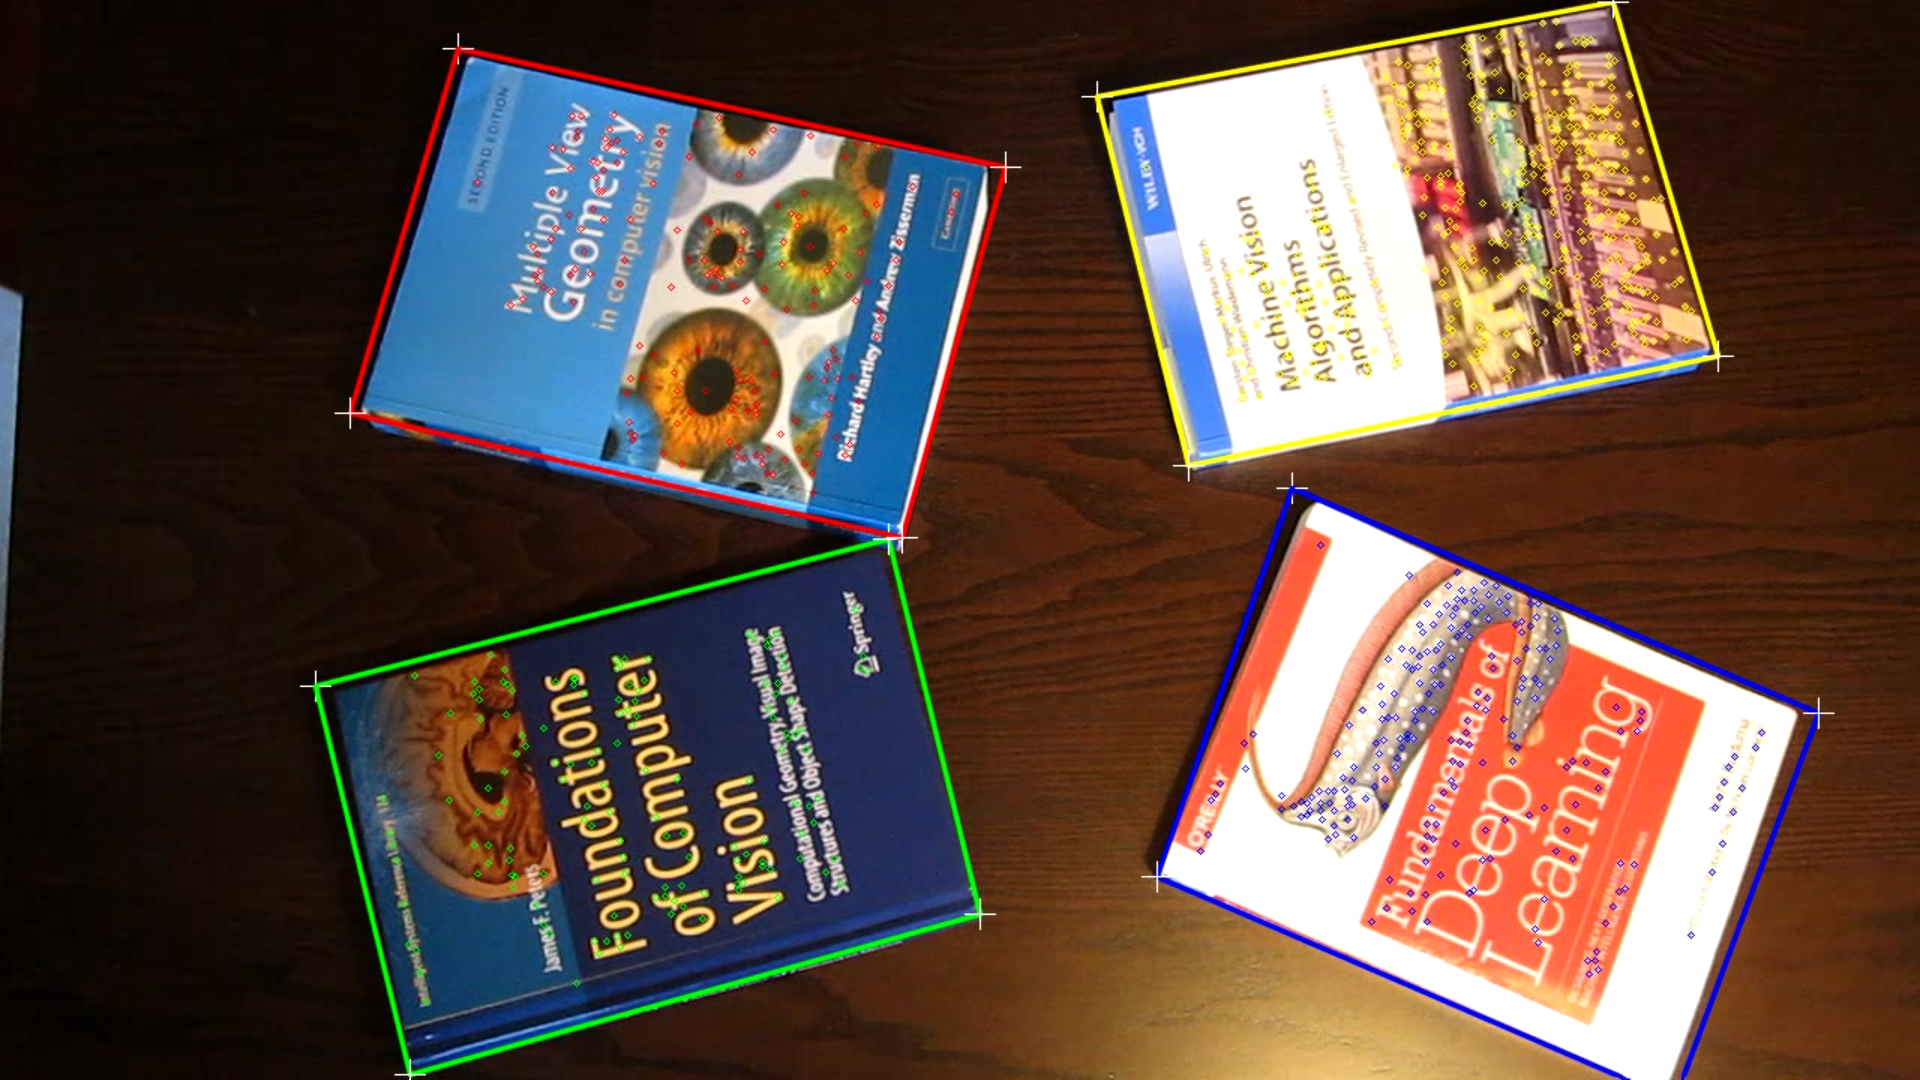
\includegraphics[scale=0.2]{Figures/output1}
\caption{An initial frame($ratio = 6$).}\label{matches1}
\end{figure}
\begin{figure}[h]
\centering
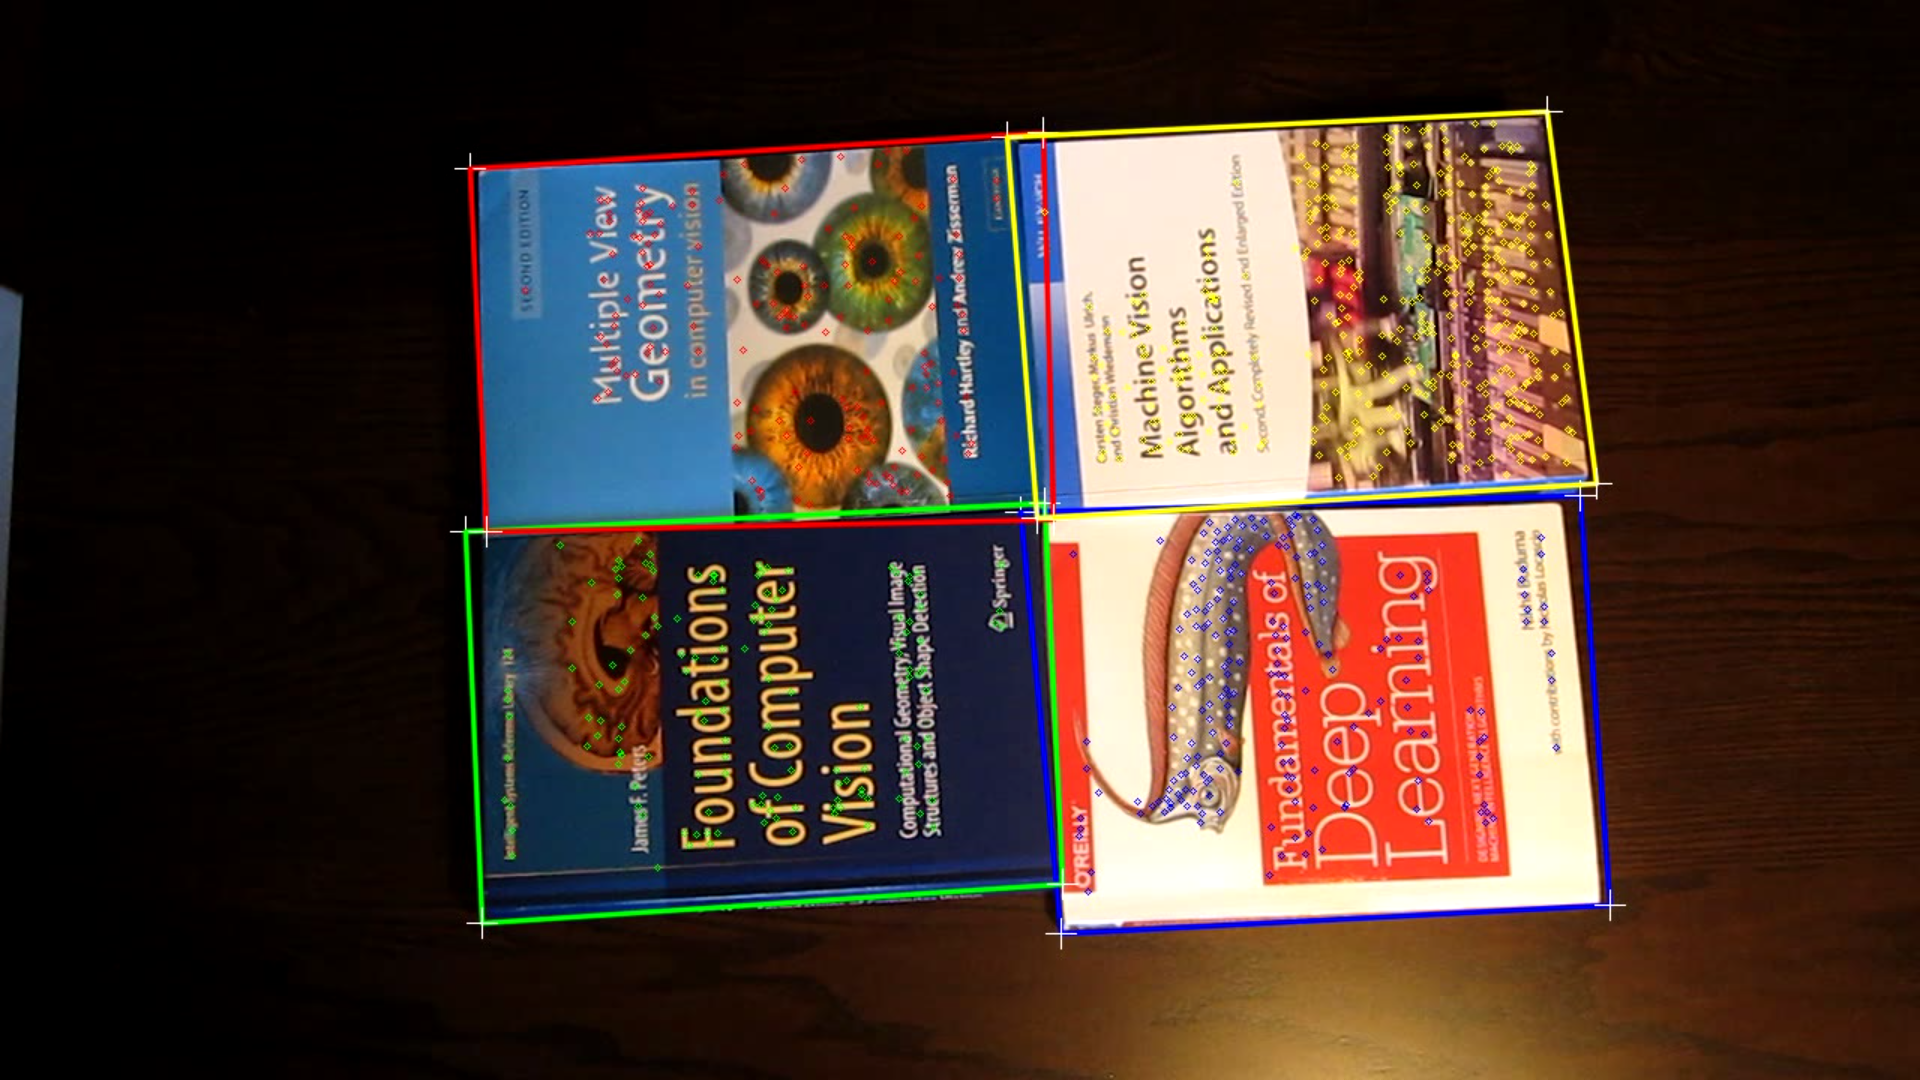
\includegraphics[scale=0.2]{Figures/output2}
\caption{An intermediate frame ($ratio = 6$).}\label{matches2}
\end{figure}
\begin{figure}[H]
\centering
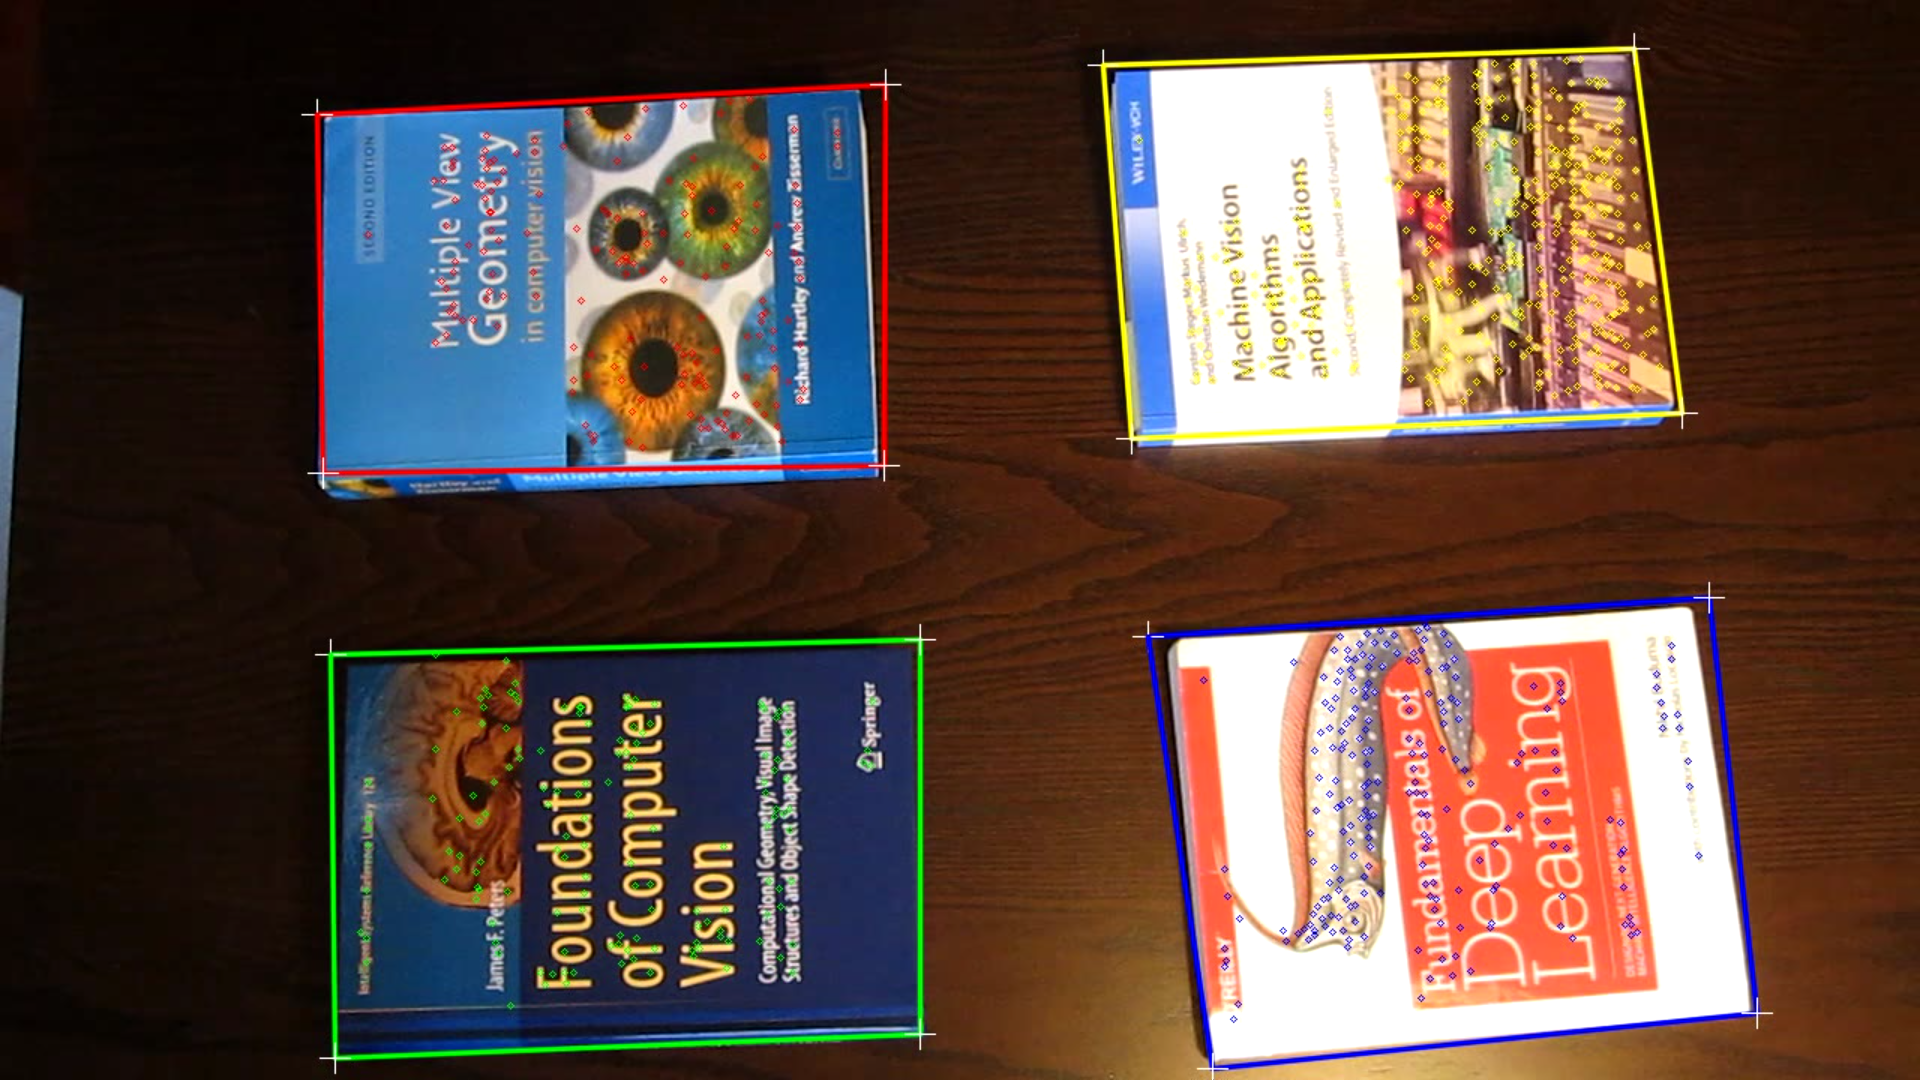
\includegraphics[scale=0.2]{Figures/output3}
\caption{A final frame ($ratio = 6$).}\label{matches3}
\end{figure}
\end{document}